\chapter{Hash Dictionaries}
\label{ch:hdict}

\newcommand{\lecnum}{13}
%\newcommand{\lectitle}{Hash Dictionaries}
\newcommand{\lecturer}{Frank Pfenning, Rob Simmons, Iliano Cervesato}

\chapterTAGS{correctness, dictionary, ds-invariant, genericity, hashing, interface, randomness, safety, set, testing}
\maketitle

\begin{preamble}
\noindent
In this lecture, we will discuss the data structure of hash tables
further and use hash tables to implement a very basic interface of
dictionaries.  With this lecture, we will also begin to discuss a new
separation of concerns. Previously, we have talked a great deal about
the distinction between a library's interface (which the client can
rely on) and a library's implementation (which should be able to
change without affecting a correctly-designed client).

The interface defines not only the \emph{types}, but also the
available \emph{operations} on them and the pre- and post-conditions
for these operations.  For general data structures it is also useful
to note the asymptotic complexity of the operations so that potential
clients can decide if the interface serves their purpose.

One wrinkle we have not yet encountered is that, in order for a
library to provide its services, it may in turn require some
operations supplied by the client.  Hash tables provide an excellent
example for this complication, so we will discuss the interface to
hash tables in details before giving the hash table implementation.

%% In this lecture, we will begin a discussion of \emph{client
%%   interfaces} -- the idea that we can write data structures that are,
%% on their own, incomplete, and that can be completed with extra
%% information from the client. Just like the library interface explains
%% the limited information that the client knows about the library's
%% implementation, the client interface explains the limited information
%% that the library knows about the client's implementation.

%% The notion of an \emph{interface} to an implementation of an abstract
%% data type or library is an extremely important concept in computer
%% science.

For the purposes of this lecture we call the data structures and the
operations on them provided by an implementation the \emph{library}
and code that uses the library the \emph{client}.
\end{preamble}


\begin{gram}[Learning Goals]
Relating to our learning goals, we have
\begin{description}

\item[Computational Thinking:] We discuss the separation of client
  interfaces and client implementations.

\item[Algorithms and Data Structures:] We discuss algorithms for
  hashing strings.

\item[Programming:] We revisit the \lstinline'char' data type and use
  it to consider string hashing.  We use this to implement a data
  structure based on a hash table.
\end{description}
\end{gram}


\section{Generic Data Structures --- I}
\label{sec:hdict:genericity}
\TAGS{genericity, interface, queue}

So far, all the data structures that we've considered, have always had
particular type information that seemed irrelevant. In the
implementation of queues, why is it important that we have a queue of
\emph{strings} in particular?
\begin{lstlisting}[language={[C0]C}]
// typedef ______* queue_t;
bool queue_empty(queue_t Q)              /* O(1) */
  /*@requires Q != NULL; @*/;
queue_t queue_new()                      /* O(1) */
  /*@ensures \result != NULL; @*/;
void enq(queue_t Q, string x)            /* O(1) */
  /*@requires Q != NULL; @*/;
string deq(queue_t S)                    /* O(1) */
  /*@requires Q != NULL && !queue_empty(S); @*/ ;
\end{lstlisting}
It's both wasteful and a potential source of errors to have to rewrite
our code if we want our program to use integers (or chars, or pointers
to structs, or arrays of strings, \ldots) instead of strings. A way we
deal with this is by creating a type, \lstinline'elem', that is used
\emph{by} the library but not defined \emph{in} the library:

\begin{lstlisting}[language={[C0]C}]
/*** Client interface ***/
// typedef _______ elem;     // Supplied by client

/*** Library interface ***/
// typedef ______* queue_t;
bool queue_empty(queue_t Q)              /* O(1) */
/*@requires Q != NULL; @*/;
queue_t queue_new()                      /* O(1) */
/*@ensures \result != NULL; @*/;
void enq(queue_t Q, elem x)              /* O(1) */
/*@requires Q != NULL; @*/;
elem deq(queue_t Q)                      /* O(1) */
/*@requires Q != NULL && !queue_empty(S); @*/ ;
\end{lstlisting}
The underscores in the library interface, before \lstinline'queue_t',
mean that the client doesn't know how the abstract type
\lstinline'queue_t' is implemented beyond knowing that it is a
pointer.  The library is therefore free to change this implementation
without breaking any (interface-respecting) client code. The
underscores in the \emph{client} interface mean that the
\emph{library} doesn't know how the abstract type \lstinline'elem' is
implemented, which means that the client is free to change this
implementation without breaking the library. The library's
implementation just refers to the \lstinline'elem' type, which it
expects the client to have already defined, whenever it needs to refer
to client data.  Therefore, the client code must be split into (at
least) two files: one, call it \lstinline'queue-client.c0', which
defines \lstinline'elem', for example as
\begin{lstlisting}[language={[C0]C}]
typedef string elem;
\end{lstlisting}
if we are interested in queues of strings, and the rest of the
program, for example \lstinline'main.c0'.  Now, if the file containing
the implementation of the queue library is called
\lstinline'queue.c0', the overall program shall be compiled as

\begin{lstlisting}[language={[coin]C}]
% cc0 queue-client.c0 queue.c0 main.c0
\end{lstlisting}
in order to respect the dependencies.

This approach is still not perfect, because any given program only
supports a single type of queue element. We'll start working on that
problem in the next lecture.

%% \section{Generic Sets and Dictionaries}

%% Hash tables are a way of implementing both \emph{sets} and
%% \emph{dictionaries}. We've seen dictionaries in a couple of settings:
%% dictionaries that map from dictionary words (the keys) and frequency
%% counts (the values), as well as from operator names (the keys) to
%% their values.





%% In a \textbf{dictionary}, we want to have some notion of what a
%% \emph{key} is and some notion of what a \emph{value} is. We want to be
%% able to insert key-value pairs into the dictionary, and we want to be
%% able to lookup which value (if any) is associated with a particular
%% key.
%% In a \textbf{set}, we don't have a separate notion of keys and
%% values. Instead, we have a single idea of an \emph{element}.

%% Sometimes the elements of a set are like examples we have already
%% seen: strings, zip codes, and so on. Sometimes, however, we think of
%% the elements of a hash set as \emph{containing} a key, and two
%% elements are \emph{equivalent} if they share the same key part --- a
%% notion that will be entirely decided by the client when they decide
%% what an element is. Our interface for sets will then give us a lookup
%% function that allows us to take an element and determine whether an
%% equivalent element already exists in the set.  As an example, the
%% elements in a set might be structs with
%% fields for a student's name, student, school, and major. If we decide that the
%% student ID is the key part, then we can look up a student's full record
%% by creating a struct that just has the correct student ID, and then
%% finding the equivalent record in the set of student records:
%% \begin{center}
%% 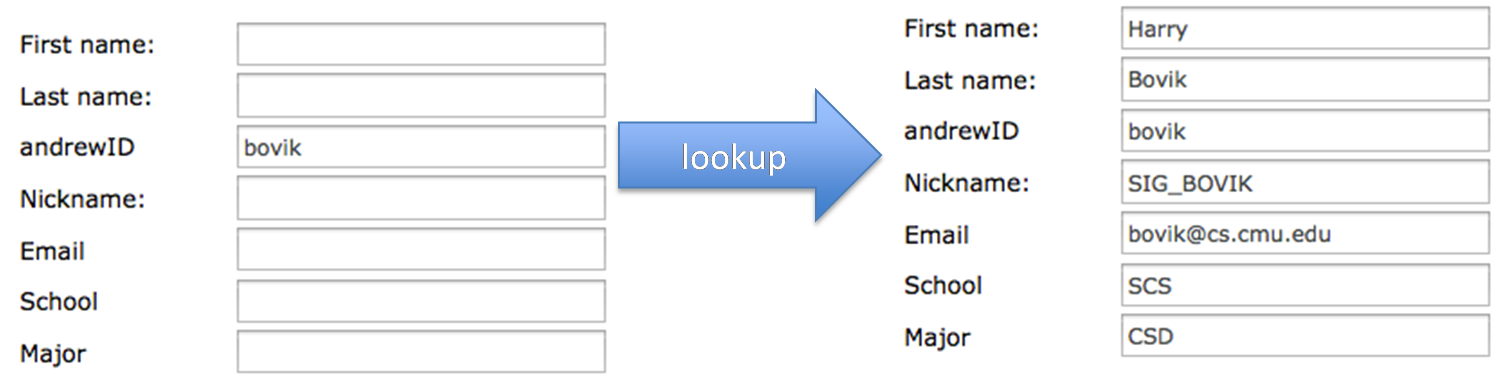
\includegraphics[width=0.99\textwidth]{img/ldap.png}
%% \end{center}


\section{Generic Hash Dictionaries}
\label{sec:hdict:generic_hash_dicts}
\TAGS{dictionary, genericity, hashing, interface}

When we implement the dictionary interface with a hash table, we'll
call it a \emph{hash dictionary} or \lstinline'hdict'.  Our hash
dictionary implementation will be \emph{generic}; it will work
regardless of the type of entries to be stored in the table as well as
of the type of their keys.

We need to think carefully about which types and functions are
provided by the client of the hash dictionary, and which are provided
by the library itself.  Clearly, the library should determine the type
of hash dictionaries:
\begin{lstlisting}[language={[C0]C}]
/* library side types */
// typedef ______* hdict_t;
\end{lstlisting}
That is really the only type provided by the implementation.  In
addition, the library interface is supposed to provide a few
functions:
\begin{lstlisting}[language={[C0]C}]
/* library side functions */
hdict_t hdict_new(int capacity)          /* O(1) */
/*@requires capacity > 0; @*/
/*@ensures \result != NULL; @*/ ;

entry hdict_lookup(hdict_t H, key k)     /* O(1) avg. */
/*@requires H != NULL; @*/ ;

void hdict_insert(hdict_t H, entry x)    /* O(1) avg. */
/*@requires H != NULL && x != NULL; @*/ ;
\end{lstlisting}
The function \lstinline'hdict_new(int capacity)' takes the initial
capacity of the hash table as an argument (which must be strictly
positive) and returns a new hash dictionary without any entry in it.

The function \lstinline'hdict_lookup(hdict_t H, key k)' answers the
question of whether an entry with key \lstinline'k' has been added to
the dictionary already and, if the answer is positive, it returns this
entry.  We will see momentarily how to express these outcomes.  This
will allows us to add postconditions that the client can use to reason
about his/her code.

The last function, \lstinline'hdict_insert(hdict_t H, entry x)', adds
entry \lstinline'x' to the dictionary.  It too will be extended with a
postcondition.

\medskip

From these decisions we can see that the \emph{client} must provide
the type of entries and the type of their keys.  Only the client can
know what these might be in any particular use of the library. In this
implementation, we don't need to know anything about the type
\lstinline'key' of keys.  We will however require entries to have
pointer type and be non-\lstinline'NULL'.  Doing so allows
\lstinline'hdict_lookup' to return \lstinline'NULL' to signal that the
dictionary does not contain any entry with the requested key.  Thus, the
client interface specifies that the following types be provided:
\begin{lstlisting}[language={[C0]C}]
/* client-side types */
// typedef ______* entry;               // Supplied by client
// typedef ______  key;                 // Supplied by client
\end{lstlisting}

Does the client also need to provide any functions?  Yes!  The hash
table implementation needs functions that can operate on values of the
types \lstinline'key' and \lstinline'entry' so that it can hash keys,
determine whether keys are equal, and extract keys from entries.
Since the library is supposed to be generic, the library implementer
cannot write these functions; we require the client to provide them.

There are three of these ``client-side'' functions.
\begin{enumerate}
\item%
  When looking up a key, it needs to match this key with the key of
  entries of interest in the dictionary.  To do so, the library needs
  a function that recovers a key from an entry:
\begin{lstlisting}[language={[C0]C}]
key entry_key(entry x)             // Supplied by client
/*@requires x != NULL; @*/ ;
\end{lstlisting}
Since \lstinline'hdict_lookup' returns \lstinline'NULL' to signal that
an entry with the requested key is not present, we disallow
\lstinline'NULL' entries.

This function allows us to provide \lstinline'hdict_insert' with a
useful postcondition: after inserting an entry, we expect to be able
to get it back when looking up its key.
\begin{lstlisting}[language={[C0]C}]
void hdict_insert(hdict_t H, entry x)
/*@requires H != NULL && x != NULL; @*/
/*@ensures hdict_lookup(H, entry_key(x)) == x; @*/ ;
\end{lstlisting}

\item%
  We also need a hash function which maps keys to integers.
\begin{lstlisting}
int key_hash(key k);               // Supplied by client
\end{lstlisting}
The result, the \emph{hash value}, can be any integer, so our hash
table implementation will have to take both this arbitrary integer and
$m$, the size of the hash table's table, into consideration when
figuring out which index of the table the key hashes to.  For the hash
table implementation to achieve its advertised (average-case)
asymptotic complexity, the resulting index should have the property
that its results are evenly distributed between $0$ and $m$.  The hash
set implementation will work correctly (albeit slowly) even if it maps
every key to $0$.

\item%
  Hash table operations also need to check for the equality of keys in
  order to be able to tell whether two objects that collide are
  actually the same or not.
\begin{lstlisting}[language={[C0]C}]
bool key_equiv(key k1, key k2);    // Supplied by client
\end{lstlisting}

With this function, we can add a postcondition to
\lstinline'hdict_lookup': either it returns \lstinline'NULL' or the
returned entry has the key we were looking for:
\begin{lstlisting}[language={[C0]C}]
entry hdict_lookup(hdict_t H, key k)
/*@requires H != NULL; @*/
/*@ensures \result == NULL
        || key_equiv(entry_key(\result), k); @*/ ;
\end{lstlisting}
\end{enumerate}

This completes the interface which we now summarize.


\begin{lstlisting}[language={[C0]C}]
/************************/
/*** Client interface ***/
/************************/

// typedef ______* entry;               // Supplied by client
// typedef ______  key;                 // Supplied by client

key  entry_key(entry x)                 // Supplied by client
  /*@requires x != NULL; @*/ ;
int  key_hash(key k);                   // Supplied by client
bool key_equiv(key k1, key k2);         // Supplied by client


/*************************/
/*** Library interface ***/
/*************************/

// typedef ______* hdict_t;

hdict_t hdict_new(int capacity)
/*@requires capacity > 0; @*/
/*@ensures \result != NULL; @*/ ;

entry hdict_lookup(hdict_t H, key k)
/*@requires H != NULL; @*/
/*@ensures \result == NULL
        || key_equiv(entry_key(\result), k); @*/ ;

void hdict_insert(hdict_t H, entry x)
/*@requires H != NULL && x != NULL; @*/
/*@ensures hdict_lookup(H, entry_key(x)) == x; @*/ ;
\end{lstlisting}

%% The function \lstinline'hdict_size' reports the total number of
%% elements in the array (remember that the load factor is the size
%% $n$ divided by the capacity $m$).  The function
%% \lstinline'ht_stats' has no effect, but prints out a histogram
%% reporting how many chains in the hash table are empty, how many
%% have length 1, how many have length 2, and so on.  For a hash table
%% to have good performance, chains should be generally short.

\clearpage
\section{A Tiny Client}
\label{sec:hdict:sample_client}
\TAGS{dictionary, genericity, hashing}

One sample application is to count word occurrences --- say, in a
corpus of Twitter data or in the collected works of Shakespeare.  In
this application, the keys are the words, represented as strings.
Entries are pairs of words and word counts, the latter represented as
integers.

\begin{lstlisting}[language={[C0]C}]
/******************************/
/* client-side implementation */
/******************************/
struct wcount {
  string word;     // key
  int count;       // other data
};

// Fulfilling the client interface
typedef struct wcount* entry;
typedef string         key;

key entry_key(entry x)
//@requires x != NULL;
{
  return x->word;
}

int key_hash(key k) {
  return hash_string(k);            /* defined below */
}

bool key_equiv(key k1, key k2) {
  return string_equal(k1, k2);
}
\end{lstlisting}


\section{A Universal Hash Function}
\label{sec:hdict:string_hashing}
\TAGS{hashing, randomness, testing}

One question we have to answer is how to hash strings, that is,
how to map strings to integers so that the integers are evenly
distributed no matter how the input strings are distributed.

We can get access to the individual characters in a string with the function
\lstinline'string_charat(s, i)', and we can get the integer ASCII value of a
\lstinline'char' with the function \lstinline'char_ord(c)'; both of these are
defined in the C0 \lstinline'string' library. Therefore, our general picture
of hashing strings looks like this:
\begin{lstlisting}[language={[C0]C}]
int hash_string(string s) {
  int len = string_length(s);
  int h = 0;
  for (int i = 0; i < len; i++)
  //@loop_invariant 0 <= i;
  {
    int ch = char_ord(string_charat(s, i));
    // Do something to combine h and ch
  }
  return h;
}
\end{lstlisting}
Now, if we don't add anything to replace the comment, the function
above will still allow the hash table to work correctly, it will just
be very slow because the hash value of every string will be zero.

A slightly better idea is combining \lstinline'h' and \lstinline'ch' with
addition or multiplication:
\begin{lstlisting}[language={[C0]C}]
  for (int i = 0; i < len; i++)
  //@loop_invariant 0 <= i;
  {
    int ch = char_ord(string_charat(s, i));
    h = h + ch;
  }
\end{lstlisting}

\noindent
This is still pretty bad, however. We can see how bad by entering the
$n = 45,600$ vocabulary words from the Collected Works of William
Shakespeare, say, into a table with $m = 22,800$ chains (load factor
is 2) and running \lstinline'ht_stats':
\begin{lstlisting}[language={[coin]C}]
Hash table distribution: how many chains have size...
...0:   21217
...1:   239
...2:   132
...3:   78
...4:   73
...5:   55
...6:   60
...7:   46
...8:   42
...9:   23
...10+: 835
Longest chain: 176
\end{lstlisting}
Most of the chains are empty, and many of the chains are very, very
long.  One problem is that most strings are likely to have very small
hash values when we use this hash function. An even bigger problem is
that rearranging the letters in a string will always produce another
string with the same hash value --- so we know that \lstinline'"cab"' and
\lstinline'"abc"' will always collide in a hash table. Hash collisions are
inevitable, but when we can easily predict that two strings have the
same hash value, we should be suspicious that something is wrong.

To address this, we can manipulate the value $h$ in some way before we
combine it with the current value. Some versions of Java use this as their
default string hashing function.
\begin{lstlisting}[language={[C0]C}]
  for (int i = 0; i < len; i++)
  //@loop_invariant 0 <= i;
  {
    int ch = char_ord(string_charat(s, i));
    h = 31*h;
    h = h + ch;
  }
\end{lstlisting}

\noindent
This does much better when we add all the vocabulary strings into the
hash table:
\begin{lstlisting}[language={[coin]C}]
Hash table distribution: how many chains have size...
...0:   3057
...1:   6210
...2:   6139
...3:   4084
...4:   2151
...5:   809
...6:   271
...7:   53
...8:   21
...9:   4
...10+: 1
Longest chain: 10
\end{lstlisting}

We can try adding a bit of randomness into this function in a number
of different ways. For instance, instead of multiplying by 31, we
could multiply by a number generated by the pseudo-random number
generator from C0's library:
\begin{lstlisting}[language={[C0]C}]
  rand_t r = init_rand(0x1337BEEF);
  for (int i = 0; i < len; i++)
    //@loop_invariant 0 <= i;
    {
      int ch = char_ord(string_charat(s, i));
      h = rand(r) * h;
      h = h + ch;
    }
  \end{lstlisting}

If we look at the performance of this function, it is comparable to
the Java hash function, though it is not actually quite as good ---
more of the chains are empty, and more are longer.
\begin{lstlisting}[language={[coin]C}]
Hash table distribution: how many chains have size...
...0:   3796
...1:   6214
...2:   5424
...3:   3589
...4:   2101
...5:   1006
...6:   455
...7:   145
...8:   48
...9:   15
...10+: 7
Longest chain: 11
\end{lstlisting}

Many other variants are possible; for instance, we could
try directly applying the linear congruential generator to the hash value
at every step:
\begin{lstlisting}[language={[C0]C}]
  for (int i = 0; i < len; i++)
    //@loop_invariant 0 <= i;
    {
      int ch = char_ord(string_charat(s, i));
      h = 1664525 * h + 1013904223;
      h = h + ch;
    }
\end{lstlisting}
The key goals are that we want a hash function that is very quick to
compute and that nevertheless achieves good distribution across our
hash table.  Handwritten hash functions often do not work well, which
can significantly affect the performance of the hash table.  Whenever
possible, the use of randomness can help to avoid any systematic bias.


\section{Coherence}
\label{sec:hdict:coherence}
\TAGS{correctness, hashing}

Recall the functions \lstinline'key_hash' and \lstinline'key_equiv' of
our tiny client:
\begin{lstlisting}[language={[C0]C}]
int key_hash(key k) {
  return hash_string(k);            /* from hash-string.c0 */
}

bool key_equiv(key k1, key k2) {
  return string_equal(k1, k2);
}
\end{lstlisting}
In this example, a key is a string.

\medskip
Consider replacing \lstinline'key_equiv' with a function that checks
that the input keys have the same length:
\begin{lstlisting}[language={[C0]C}]
bool key_equiv(key k1, key k2) {
  return string_length(k1) == string_length(k2);
}
\end{lstlisting}
This does not feel right.  Let's see what would happen when we use
this \lstinline'key_equiv' and our original \lstinline'key_hash' in
our hash dictionary.  After populating it with a large corpus, for
example the works of William Shakespeare, assume we lookup a
misspelled word, for example \lstinline'"amlet"'.  The function
\lstinline'key_hash' will convert it to a hash value which will be
used to compute the index of a chain.  If this chain contains an entry
whose key has length 5 (the length of \lstinline'"amlet"'), it will
return this entry, although its key is not \lstinline'"amlet"'!  This
result is incorrect.

In a well-designed hash table, keys that are considered equal should
hash to the same value, a condition we call \emph{coherence}.  As we
just saw, whenever the hashing and the equivalence functions are
incoherent, there is the concrete risk of our hash dictionaries
working incorrectly.

\medskip
What if we weaken the hash function instead of the equality check?
Consider now our original \lstinline'key_equiv' and a hash function
that returns the ASCII code of the first letter of its input (or 0
when passed the empty string):
\begin{lstlisting}[language={[C0]C}]
int key_hash(key k) {
  if (string_equal(k, "") return 0
  return char_ord(string_charat(k, 0));
}
\end{lstlisting}
Then every word starting with the same letter will have the same hash
value, and therefore will end up at the same table index.  Its chains
will be very long for a large dictionary, while other indices will
be empty.  When looking up a word, once on the appropriate chain,
\lstinline'key_equiv' will correctly either find it or report that it
is not in the dictionary.  The issue here is performance, not
correctness: this choice leads to long chains and therefore slow
searches.

The problem with both of these setups is that \lstinline'key_hash' and
\lstinline'key_equiv' used the information in the key in very
different measures.  Instead, our original choices were very much in
harmony.


\section{A Fixed-Size Implementation of Hash Tables}
\label{sec:hdict:hash_dict_impl}
\TAGS{correctness, dictionary, ds-invariant, hashing, safety}

For simplicity, we will now write a non-resizing implementation of
hash dictionaries.  We leave it as an exercise to modify this code to
use unbounded arrays to support on-demand resizing of the table.

A non-resizing implementation requires that we can a priori predict a
good size, or we will not be able to get the advertised $O(1)$ average
time complexity.  Choose the size too large and it wastes space and
slows the program down due to a lack of locality.  Choose the size too
small and the load factor will be high, leading to poor asymptotic
(and practical) running time.

We start with the type of lists to represent the chains of entries,
and the hash table type itself.
\begin{lstlisting}[language={[C0]C}]
/*******************************/
/* library-side implementation */
/*******************************/
typedef struct chain_node chain;
struct chain_node {
  entry data;              // != NULL
  chain* next;
};

typedef struct hdict_header hdict;
struct hdict_header {
  int size;                 // 0 <= size
  int capacity;             // 0 < capacity
  chain*[] table;           // \length(table) == capacity
};
\end{lstlisting}
The first thing after the definition of a data structure is a function
to verify its invariants.  Besides the invariants noted above we
should check
% that each data value in each chain in the hash table should be non-null and
the hash value of the key of every entry in each chain stored in
$A[i]$ is indeed $i$. (This \lstinline'is_hdict' function is
incomplete.)

\begin{lstlisting}[language={[C0]C}]
bool is_hdict(hdict* H) {
  return H != NULL
      && 0 <= H->size
      && 0 < H->capacity
      && is_array_expected_length(H->table, H->capacity);
   /* && there are no NULL entries */
   /* && each entry satisfies its own representation invariants */
   /* && there aren't entries with equal key */
   /* && the number of entries matches the size */
   /* && every entry in H->table[i] hashes to i */
   /* && ... */
}
\end{lstlisting}
Recall that the test on the length of the array must be inside an
annotation, because the \length{} function is not available when
the code is compiled without dynamic checking enabled.

In order to check that the keys in a hash dictionary hash to the correct
index, we need a way of mapping the hash value returned by
\lstinline'key_hash' to an index of the table.  This is a common enough
operation that we'll write a helper function:
\begin{lstlisting}[language={[C0]C}]
int index_of_key(hdict* H, key k)
//@requires is_hdict(H);
//@ensures 0 <= \result && \result < H->capacity;
{
  return abs(key_hash(k) % H->capacity);
}
\end{lstlisting}

Allocating a hash table is straightforward.
\begin{lstlisting}[language={[C0]C}]
hdict* hdict_new(int capacity)
//@requires capacity > 0;
//@ensures is_hdict(\result);
{
  hdict* H = alloc(hdict);
  H->size = 0;
  H->capacity = capacity;
  H->table = alloc_array(chain*, capacity);
  return H;
}
\end{lstlisting}
Equally straightforward is searching for an entry with a given key.
We omit the standard loop invariant.
\begin{lstlisting}[language={[C0]C}]
entry hdict_lookup(hdict* H, key k)
//@requires is_hdict(H);
//@ensures \result == NULL || key_equiv(entry_key(\result), k);
{
  int i = index_of_key(H, k);
  for (chain* p = H->table[i]; p != NULL; p = p->next) {
    if (key_equiv(entry_key(p->data), k))
      return p->data;
  }
  return NULL;
}
\end{lstlisting}

Inserting an entry follows generally the same structure
as search.  If we find an entry in the correct chain with the
same key we replace it.  If we find none, we insert a new
node at the beginning of the chain.
\begin{lstlisting}[language={[C0]C}]
void hdict_insert(hdict* H, entry x)
//@requires is_hdict(H);
//@requires x != NULL;
//@ensures is_hdict(H);
//@ensures x == hdict_lookup(H, entry_key(x));
{
  key k = entry_key(x);
  int i = index_of_key(H, k);
  for (chain* p = H->table[i]; p != NULL; p = p->next) {
    //@assert p->data != NULL; // Not given by loop invariant!
    if (key_equiv(entry_key(p->data), k)) {
      p->data = x;
      return;
    }
  }

  // prepend new entry
  chain* p = alloc(chain);
  p->data = x;
  p->next = H->table[i];
  H->table[i] = p;
  (H->size)++;
}
\end{lstlisting}


\section{Hash Sets}
\label{sec:hdict:hash_sets}
\TAGS{hashing, interface, set}

A \emph{set} is a collection of elements without duplicates.
Elementary operations we will be interested in are inserting an
element into a set and asking whether an element is a member of a set.

The basic technology of hash table can also be leveraged to give an
efficient implementation of sets.  Specifically, we can think of a set
as a dictionary where both keys and entries are the elements.  This
allows us to simplify and specialize the hash dictionary interface
into a hash set interface which provides the abstract type
\lstinline'hset' and the above operations.
\begin{itemize}
\item%
  We collapse the types \lstinline'key' and \lstinline'entry' into a
  single type that we call \lstinline'elem'.
\item%
  Extracting a key from an entry becomes vacuous.  Consequently we can
  do without an \lstinline'entry_key' function.
\item%
  The lookup function of dictionaries underlies a membership test: it
  returns \lstinline'NULL' if the element is not in the set, and the
  element itself if it is.  We can streamline this behavior by having
  the hash set version, which we call \lstinline'hset_contains',
  return a boolean.  This also lets us do without the requirement that
  the data contained in the hash table be a pointer type:
  \lstinline'elem' can be any type.
\end{itemize}

The resulting interface for hash sets is as follows:
\begin{lstlisting}[language={[C0]C}]
/************************/
/*** Client interface ***/
/************************/

// typedef _______ elem;           // Supplied by client
bool elem_equiv(elem x, elem y);   // Supplied by client
int elem_hash(elem x);             // Supplied by client

/*************************/
/*** Library interface ***/
/*************************/

// typedef ______* hset_t;

hset_t hset_new(int capacity)          /* O(1) */
/*@requires capacity > 0; @*/
/*@ensures \result != NULL; @*/ ;

bool hset_contains(hset_t H, elem x)   /* O(1) avg. */
/*@requires H != NULL; @*/ ;

void hset_add(hset_t H, elem x)        /* O(1) avg. */
/*@requires H != NULL; @*/
/*@ensures hset_contains(H, x); @*/ ;
\end{lstlisting}



\clearpage
\section{Exercises}
\label{sec:hdict:exercises}

\begin{flex}
\begin{exercise}[\opt{sample solution on page~\pageref{ex:hdict_student-dict-solved}}]
\label{ex:hdict_student-dict}
  We want to use the hash dictionaries developed in this chapter to
  keep track of grades and other student data, and access them by
  student id.  A student id is an integer and the associated grades
  are a stored in a character array of some fixed length tracked
  outside the hash dictionary.  A student record also includes notes
  about the student (a string) and whether this student is auditing
  the course (a boolean).

  Implement the client interface of hash dictionaries by defining the
  types \lstinline'entry' and \lstinline'key' and the functions
  \lstinline'entry_key', \lstinline'key_hash' and
  \lstinline'key_equiv'.
\end{exercise}

\begin{lrbox}{0\null\global\setbox\lstbox}
\begin{lstlisting}[language={[C0]C}]
struct  student_record {
  int student_id;
  char[] grades;
  string notes;
  bool auditor;
};

typedef struct student_record* entry;
typedef int key;

key entry_key(entry x)
//@requires x != NULL;
{
  return x->student_id;
}

int key_hash(key k) {
  return hash_int(k);
}

bool key_equiv(key k1, key k2) {
  return k1 == k2;
}
\end{lstlisting}
\end{lrbox}

\begin{solution}\opt{\textbf{of exercise~\ref{ex:hdict_student-dict}}}
\label{ex:hdict_student-dict-solved}
This solution assumes that we have written a function
\lstinline'hash_int' that maps integers to values uniformly
distributed over the range of all C0 integers.
%% Pulled out in \lstbox to support fancy solutions
% \begin{lstlisting}[language={[C0]C}]
% struct  student_record {
%   int student_id;
%   char[] grades;
%   string notes;
%   bool auditor;
% };

% typedef struct student_record* entry;
% typedef int key;

% key entry_key(entry x)
% //@requires x != NULL;
% {
%   return x->student_id;
% }

% int key_hash(key k) {
%   return hash_int(k);
% }

% bool key_equiv(key k1, key k2) {
%   return k1 == k2;
% }
% \end{lstlisting}
\par\medskip\noindent\usebox{\lstbox}\par
\end{solution}
\end{flex}


\begin{flex}
\begin{exercise}[\opt{sample solution on page~\pageref{ex:hdict_tabulate-solved}}]
\label{ex:hdict_tabulate}
We are extending the hash table interface with a new function
\begin{lstlisting}[language={[C0]C}]
entry[] hdict_tabulate(hdict* H)
/*@requires H != NULL; @*/ ;
\end{lstlisting}
that returns an array with all the entries in the hash table, in some
order of your choice.  Include contracts and annotations as appropriate.
\end{exercise}

\begin{lrbox}{0\null\global\setbox\lstbox}
\begin{lstlisting}[language={[C0]C}]
entry[] hdict_tabulate(hdict* H)
//@requires is_hdict(H);
//@ensures is_hdict(H) && \length(\result) == H->size;
{
  entry[] result = alloc_array(entry, H->size);
  int j = 0;  // indexes result

  for (int i = 0; i < H->capacity; i++)
  //@loop_invariant 0 <= i && i <= H->capacity;
  {
    for (chain* p = H->table[i]; p != NULL; p = p->next)
    //@loop_invariant 0 <= j && j <= H->size;
    {
      result[j] = p->data;
      j++;
    }
  }
  return result;
}
\end{lstlisting}
\end{lrbox}

\begin{solution}\opt{\textbf{of exercise~\ref{ex:hdict_tabulate}}}
\label{ex:hdict_tabulate-solved}
%% Pulled out in \lstbox to support fancy solutions
% \begin{lstlisting}[language={[C0]C}]
% entry[] hdict_tabulate(hdict* H)
% //@requires is_hdict(H);
% //@ensures is_hdict(H) && \length(\result) == H->size;
% {
%   entry[] result = alloc_array(entry, H->size);
%   int j = 0;  // indexes result

%   for (int i = 0; i < H->capacity; i++)
%   //@loop_invariant 0 <= i && i <= H->capacity;
%   {
%     for (chain* p = H->table[i]; p != NULL; p = p->next)
%     //@loop_invariant 0 <= j && j <= H->size;
%     {
%       result[j] = p->data;
%       j++;
%     }
%   }
%   return result;
% }
% \end{lstlisting}
\par\medskip\noindent\usebox{\lstbox}\par
\end{solution}
\end{flex}


\begin{exercise}
  Extend the hash table implementation so it dynamically resizes
  itself when the load factor exceeds a certain threshold.  When
  doubling the size of the hash table you will need to explicitly
  insert every entry from the old hash table into the new one,
  because the result of hashing depends on the size of the hash table.
\end{exercise}

\begin{exercise}
  Redo the library implementation for a different client interface
  that has a function \lstinline'key_hash(key k, int m)' that returns
  a result between 0 (inclusive) and \lstinline'm' (exclusive).
\end{exercise}

\begin{exercise}
  Extend the hash table interface with a new function
  \lstinline'hdict_tabulate' that returns an array with the entries in
  the hash table, in some order of your choice.
\end{exercise}

%% \begin{exercise}
%%   Complete the client-side code to build a hash table containing word
%%   frequencies for the words appearing in Shakespeare's collected
%%   works.  You should build upon the code in Assignment 2.
%% \end{exercise}

\begin{exercise}
  Extend the hash table interface with a new function to delete the
  entry with a given key if present in the table.  To be extra
  ambitious, shrink the size of the hash table once the load factor
  drops below some minimum, similarly to the way we could grow and
  shrink unbounded arrays.
\end{exercise}

\begin{exercise}
  The hash dictionaries in this lecture relied on entries embedding
  their keys (which we retrieved with the function
  \lstinline'entry_key').  A different design is for the hash table to
  implement a mapping from keys to \emph{values}, where values do not
  embed the key.  The interface of such hash dictionaries is
\begin{lstlisting}[language={[C0]C}]
/************************/
/*** Client interface ***/
/************************/

// typedef _______ key;         // Supplied by client
// typedef _______ *value;      // Supplied by client
bool key_equiv(key x, key y);   // Supplied by client
int key_hash(key x);            // Supplied by client

/*************************/
/*** Library interface ***/
/*************************/

// typedef ______* hdict_t;

hdict_t hdict_new(int capacity)
/*@requires capacity > 0; @*/
/*@ensures \result != NULL; @*/ ;

value hdict_lookup(hdict_t H, key k)
/*@requires H != NULL; @*/ ;

void hdict_insert(hdict_t H, key k, value v)
/*@requires H != NULL; @*/
/*@requires v != NULL; @*/
/*@ensures hdict_lookup(H, k) == v; @*/ ;
\end{lstlisting}
  In particular, \lstinline'hdict_insert' takes both a key and a value
  as parameters.

  Implement this interface.
\end{exercise}

\begin{exercise}
  Write an implementation of hash sets based on the interface provided
  in this chapter.
\end{exercise}


\printsolutions
% \clearpage
% \bibliographystyle{alpha}
% \bibliography{modal}
